\documentclass[11pt, preprint]{aastex}
%%%%%%begin preamble
\usepackage[hmargin=1in, vmargin=1in]{geometry} % Margins
\usepackage{hyperref}
\usepackage{url}
\usepackage{natbib}
\setlength{\bibsep}{0pt plus 0.3ex}
\usepackage{graphicx}
\usepackage{amsmath}
\usepackage{amsfonts}
\usepackage{amssymb}
\usepackage{pdfpages} % breaks with aastex6
\usepackage{import}
\usepackage{wrapfig}

\usepackage{color}
\hypersetup{
  colorlinks   = true,
  %citecolor    = blue
  citecolor    = gray
  % gray is not being found!?!
  % gray is found if pdfpages is used... crap.
  %citecolor    = grey
  %citecolor    = Gray
}

\setcounter{tocdepth}{2}
%% headers
\usepackage{fancyhdr}
\pagestyle{fancy}
\fancyhf{} % sets both header and footer to nothing
\lhead{Evan Anders -- Research Proposal}
\rhead{Princeton Center for Theoretical Science}
\cfoot{\footnotesize{\thepage}}
%\pagestyle{empty}
%\pagenumbering{gobble}
%\renewcommand*{\thefootnote}{\fnsymbol{footnote}}

\renewcommand{\vec}{\ensuremath{\boldsymbol}}
\newcommand{\dedalus}{\href{http://dedalus-project.org}{Dedalus}}
\newcommand{\del}{\ensuremath{\vec{\nabla}}}
\newcommand{\scrS}{\ensuremath{\mathcal{S}}}

\newcommand{\nosection}[1]{%
  \refstepcounter{section}%
  \addcontentsline{toc}{section}{\protect\numberline{\thesection}#1}%
  \markright{#1}}
\newcommand{\nosubsection}[1]{%
  \refstepcounter{subsection}%
  \addcontentsline{toc}{subsection}{\protect\numberline{\thesubsection}#1}%
  \markright{#1}}

%\usepackage{atbegshi}
%%%%%%end preamble


\begin{document}
Stars like the Sun rely on vigorous near-surface convective regions to transport out the heat generated in their cores.
This convection generates sound waves which deflect due to density stratification as they propagate into the stellar interior.
The relatively new fields of helio- and asteroseismology measure those sound waves to look into the interior of the Sun and other stars.
These measurements enable the precise determination of age, mass, and radius of other stars, and have revealed the interior structure and mean flows of the Sun.
These helioseismic observations, as well as direct measurements of the Sun's surface, have been unable to detect theorized large-scale convective flows called ``giant cells.''
The absence of these flows have called into question our most fundamental understanding of the nature of convection in stars, a problem widely referred to as the ``Solar Convective Conundrum.''

State-of-the-art codes which generate profiles of the internal structure of stars often rely on one-dimensional (1D) parameterizations of convection.
These stellar structure models are used widely across many subfields of astrophysics, including asteroseismology.
Unfortunately, the 1D parameterizations that inform these codes assume giant cells exist in the Sun; this assumption conflicts with modern observations.

My research aims to  help solve this Convective Conundrum by gaining a better understanding of convection in the highly stratified, rotational, magnetized context of stellar convection.
While I draw my inspiration from problems facing the solar and stellar community, similar flow processes are important in the atmospheres and cores of planets like Jupiter and the Earth. 

\vspace{-14pt}
\section{Convection at the smallest scale: studies of individual downflows}
\vspace{-6pt}

In the presence of an atmospheric density stratification, convective flows experience a breaking of symmetry.
Slow, broad upwellings balance downflows which are intense, fast, and narrow.
It has been suggested that in the context of solar-like convection, these intense downflows are so powerful that they do not require their upflow counterpart to carry out the Sun's luminosity.
This ``entropy rain'' hypothesis, first suggested by \citet{spruit1997}, is gaining traction, and could explain the
\begin{wrapfigure}{r}{0.4\textwidth}
	\begin{center}
	\vspace{-10pt}
    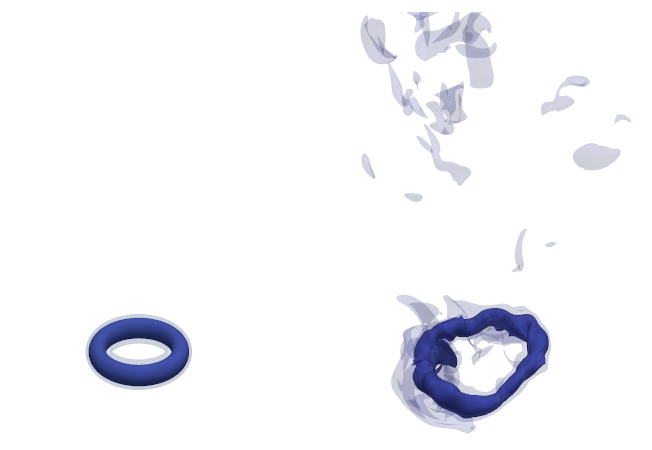
\includegraphics[width=0.38\textwidth]{./figs/thermals_comparison.png}
	\vspace{-16pt}
	\end{center}
    \caption{
	3D visualizations of the entropy perturbation of evolved thermals in the laminar (left) and turbulent (right) regimes.
	\label{fig:thermals_comparison} }
	\vspace{-11pt}
\end{wrapfigure}
lack of giant cells in observations \citep{hanasoge&all2015}.
Recent simulations of solar-like convection suggest that surface-driven downflows can indeed transport most of the Sun's luminosity \citep{kapyla&all2017}, and recent theoretical work showed that such a concept could be included into 1D parameterizations \citep{brandenburg2016}.
These modern results suggest that stellar downflows deserve more careful study.
It is possible these downflows turbulently break up into distinct pieces as they fall and these individual downflow pieces can be well modeled as ``thermals.''
Thermals are regions of cold fluid which accelerate due to buoyancy forces and shape themselves into vortex rings; evolved thermals are visualized in Fig. \ref{fig:thermals_comparison}.
Thermals are also observed and studied in the Earth's atmosphere \citep{lecoanet&jeevanjee2019}.

Over the course of my graduate studies, I have become proficient at using the open-source Dedalus \citep{burns&all2019} code to answer questions about stellar convection at various scales.
During my PhD, I used Dedalus to study thermals-as-downflows by coming to understand how atmospheric stratification affects these downflows as they fall \citep{andersLB2019}.
We surprisingly found that solar downflows could feasibly transport the solar luminosity without any help from warm upflows, giving credence to the entropy rain hypothesis.
However, these studies neglected some key ingredients in stellar convection: turbulence, magnetism, and rotation.

As a PCTS fellow, I will build upon this study from my thesis work to understand if entropy rain is feasible by including solar-like complications.
Rotation, magnetism, and turbulence could all have filtering effects on downflows, preventing their successful transit of the solar convection zone in certain regimes.
I will determine whether strong magnetic fields and global angular frequencies can ``evaporate'' entropy rain.
While \citet{lecoanet&jeevanjee2019} found that turbulence had little effect on the evolution of thermals in unstratified atmospheres, the compressional effects of atmospheric stratification could change this outcome, and I will explore this possibility.
Understanding if the inclusion of these realistic effects prevents downflows from crossing the solar convection zone will help determine the validity of the entropy rain hypothesis.
As in \citet{andersLB2019}, these studies will include both analytical and numerical analysis.
I look forward to collaborating with experts in Princeton's Geophysical Fluid Dynamics laboratory, such as Drs.~Jeevanjee and Donner, who study convection in the context of Earth's atmosphere where thermals are observed, as well as astrophysical fluid dynamicists like Prof.~Jeremy Goodman.

\vspace{-0.8cm}
\section{Mesoscale convection: interactions at the radiative-convective boundary}
\vspace{-0.3cm}
\label{sct:taskB}
\begin{figure*}[t!]
    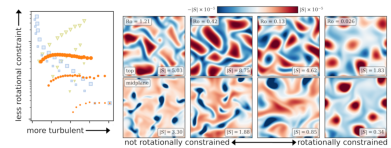
\includegraphics[width=\textwidth]{./figs/rossby_plot.png}
    \caption{(left, Fig 1b of \citet{anders&all2019}) The importance of rotation is difficult to predict as turbulence is increased in convective simulations.
	Rotational influence varies greatly along traditional paths through parameter space (green triangles and blue squares).
	We have discovered a new parameter (orange circles) that allows rotational influence to be specified \emph{a priori}.
	(right eight panels, Fig. 2 of \citet{anders&all2019}) As rotational constraint increases (from left to right), convective flows appear strikingly different and vary less as a function of height (top compared to bottom).
	It is crucial to simulate solar convection under the same rotational influence as the real Sun to ensure that flow topologies and interactions are an accurate model.
	\label{fig:rossby_plot} }
\end{figure*}

In Sun-like stars, a stably stratified ``radiative zone'' where radiation effectively carries out the Sun's heat lies beneath the turbulent surface convection zone.
In the Sun, the radiative-convective boundary (RCB) is characterized by a transition from moderate instability to strong stability.
The solar RCB furthermore coincides with a region of intense shear in the Sun's radial velocity profile called the tachocline, and it is thought that these shear interactions are a crucial driver of the Sun's magnetic dynamo.
Understanding how downflows pump angular momentum and magnetism into the RCB is a crucial to figuring out how the solar dynamo is driven, and how the tachocline was established.
Measurements suggest that the RCB is thin \citep{basu1997}, but many modern simulations produce RCBs which are up to an order of magnitude thicker than the solar one \citep{hotta2017}.
This suggests that many simulations are studying angular momentum and magnetic field pumping mechanisms in the wrong regime of ``stiffness'' of the RCB \citep{couston&all2017}.

In creating simulations of solar convection, it is important to strive to produce flows which feel the same influence of rotation and magnetism as those in the Sun.
Simulations which include global rotation can be run in regimes where flows are heavily affected by Coriolis forces or regimes where this effect is weak.
A ``critical'' rotational frequency separates these two regimes, but determining this critical frequency is often not straightforward.
During my PhD, I found a method for determining this critical frequency so that the importance of rotation could be specified in simulation initial conditions \citep[see Fig. \ref{fig:rossby_plot}a and][]{anders&all2019}.
Flows look very different depending on whether you simulate above, at, or near this critical frequency (Fig.~\ref{fig:rossby_plot}b), and it is crucial to simulate in the same regime as the Sun.
In magnetized systems, there is an analagous critical magnetic field, but to date no study has determined how to determine this field before simulation startup.

During my time at PCTS, I will study interactions between downflows and a solar-like RCB at the mesoscale in the presence of solar-like rotation and magnetism.
In order to achieve this, I will first determine the critical magnetic field using similar techniques to those that I used during my graduate career while finding the critical rotational frequency.
After determining this, I will set up solar-like rotating magnetoconvection simulations and determine if downflows can effectively pump magnetic fields and angular velocity into a thin, solar-like RCB.
I look forward to collaborating with experts in astrophysical fluid dynamics at Princeton and the IAS like Profs.~Jim Stone and Matthew Kunz on this project.

\section{Global scale convection: dynamics in relaxed atmospheres}
Modern 1D stellar models often employ the decades-old convective parameterization of mixing length theory \citep{bohm-vitense1958}, which has many deficiencies.
These deficiencies have led some researchers to seek out ways to couple one-dimensional (1D) models with fully convective, three-dimensional (3D) global simulations.
Such a coupling has recently been performed with some success \citep{jorgensen&weiss2019}.
However, these studies have thusfar only been able to couple previously computed 3D sims with 1D models, rather than coupling the two at runtime, largely because 3D simulations are costly.
Some of these costs are unavoidable: highly resolved, turbulent simulations necessarily take small timesteps, and therefore simulation times are very long.
However, some of the expense of these simulations is often time wasted waiting for the atmospheric structure and mean flows to converge to an equilibrium state, and this expense can be minimized.

\begin{wrapfigure}{r}{0.3\textwidth}
	\begin{center}
	\vspace{-10pt}
    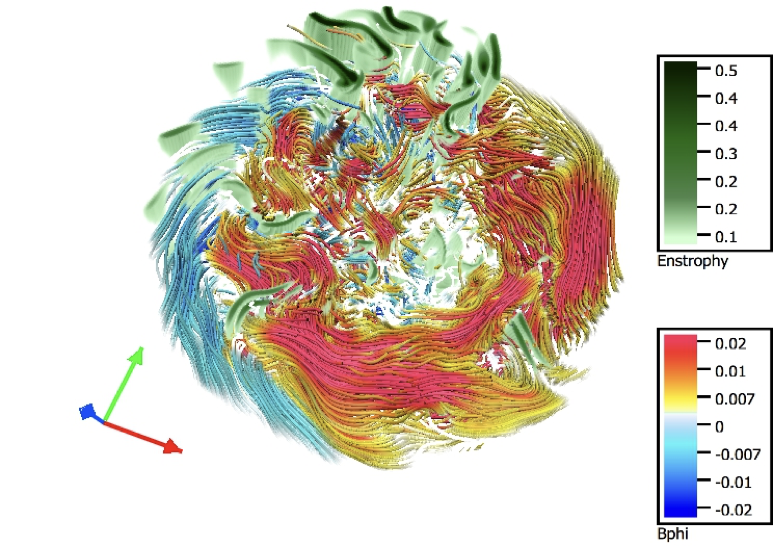
\includegraphics[width=0.28\textwidth]{./figs/mdwarf.png}
	\vspace{-16pt}
	\end{center}
    \caption{A volume rendering of a global dynamo simulation in Dedalus.
	Enstrophy, or the magnitude of vorticity, is shown in green.
	Red and blue lines denote the magnitude and direction of azimuthal magnetic field.
	\label{fig:mdwarf} }
\end{wrapfigure}
During my graduate career, I created and verified a tool for accelerating the long thermal relaxation timescale in convective systems \citep{anders&all2018}.
This tool reached a relaxed state using an order of magnitude fewer computational resources than a simulation which computes a full Kelvin-Helmholtz relaxation timescale, and results between the simulations differed by less than 1\%.

During my time at PCTS, I will extend my accelerated evolution method to the evolution of thermodynamic and angular momentum profiles in global simulations.
The tools to perform global simulations in Dedalus already exist \citep{lecoanet&all2018} and have been tested; a visualization of basic outputs from these simulations is shown in Fig.~\ref{fig:mdwarf}.
The large-scale structures seen in Fig.~\ref{fig:mdwarf} arise quickly, but the equilibration and saturation of these structures and other simulation measurements often takes timescales which are too long to feasibly simulate.
I will design a general, public module which can flexibly interact with arbitrary simulation data which reads in statistical measures of a global convection simulation and outputs the properly accelerated profile and mean flows.
This tool will allow users of codes including and beyond Dedalus to achieve rapidly relaxed states and computational speed-ups while simulating state-of-the-art turbulent dynamics.
Such a tool will benefit diverse fields of simulators, such as those who study global circulation models in the atmospheres of the Earth and exoplanets, as well as dynamo processes in planetary cores and stellar atmospheres.
Once completed, I will use this tool in my own work to accelerate the evolution of highly turbulent, solar-like simulations to understand the nature of global flows and dynamos in an equilibrated simulation.
I look forward to collaborating on this project with GFDL's experts who have sought to improve Earth-system convective parameterizations like Dr.~Silvers.


\vspace{-0.8cm}
\section{Summary}
\vspace{-0.3cm}
The Princeton Center for Theoretical Science postdoctoral fellowship would give me the freedom to study these ambitious problems in astrophysical fluid dynamics.
The projects presented here help solve exciting problems in stellar structure and will have impactful results on a variety of astrophysical disciplines.
My PhD work has excellently prepared me to tackle these problems which seek to understand stellar convection from the smallest to global scales.
Princeton is the perfect location for carrying out this work due to the opportunities available for interdisciplinary collaboration between astrophysicists, geophysical fluid dynamicists, and applied mathematicians.
I look forward to joining the center, creating cross-disciplinary collaborations, and carrying on Princeton's excellent research tradition while making lasting contributions which help solve the Convective Conundrum and other fascinating problems. 

\newpage
\bibliographystyle{apj_title}
\bibliography{biblio}
\end{document}
